\section{Core Protocol}
\label{sec:coreprotocol}

\stzh{In this section, we consider two users of our service Alice and Bob. } Alice wants to message Bob over an untrusted network, without leaking any data or metadata to anyone. To hide the message content they just use end-to-end encryption. To hide metadata they employ two key ideas: sending data at a constant rate, and retrieving homomorphically compressed data.

When signing up, each user gets their own \textit{outbox} on the server. This outbox is a dedicated storage space that the user sends messages to. Once every minute, Alice will send exactly 1 KB of data to her outbox on the server. If she has a message to send, she sends the \stzh{padded} encryption of that message, and if she has no message to send, she sends a random sequence of bytes.\stzh{A random message encrypted with a random public key?} With this simple first idea, no one, including the server and any network observers, will know when Alice actually sends a message.

The message needs to be routed to Bob. Now, a traditional messaging system would have Bob download data from Alice's outbox, and then try to decrypt it to see if it was meant for him. But this leaks metadata: the server would know that Alice wrote to outbox $x$ and that Bob read from outbox $x$, which links the two of them together!

Our solution is for Bob to, once every minute, download \textit{all} outboxes from the server. On his own computer, he can then check Alice's outbox. This way, no one, not even the server, has any way of linking Alice to Bob. All metadata is protected.

This is how Anysphere works. Obviously, Bob cannot download all outboxes every minute — that would be way too much data! — so instead he uses \textit{private information retrieval}, a well-studied cryptographic primitive, as a way of compressing his download size. The following subsections will describe the system in detail.

\begin{figure}
    \centering
    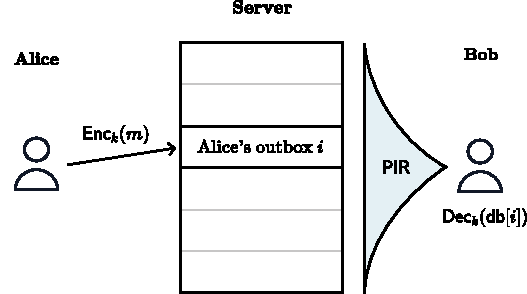
\includegraphics[width=0.4\textwidth]{pirfigure.pdf}
\caption{Alice sends to her outbox once every minute. Bob retrieves Alice's outbox using private information retrieval (PIR), which looks the same to everyone else as if he had downloaded the entire database. Alice and Bob can use standard symmetric encryption to communicate, and no one, not even the server, will learn anything at all.}
\end{figure}



\subsection{Private information retrieval}

Bob wants to download outbox $i$ without revealing $i$ to anyone. Viewing the collection of outboxes as a database array $\db$, he wants to retrieve $\db[i]$ privately. This problem was first introduced as \textit{private information retrieval} (PIR) in 1995 \cite{chor1995private}, extended in 1997 to our threat model under the name cPIR \cite{kushilevitz1997replication}, and has been extensively studied since then \cite{melchor2016xpir,angel2018pir, ahmad2021addra}.

Our implementation currently uses FastPIR, which is one of the fastest cPIR schemes \cite{ahmad2021addra}. All cPIR schemes have the same security properties (i.e., they leak zero information), and we are actively researching faster schemes (see \cref{sec:future}).

All known cPIR schemes use homomorphic encryption \cite{gentry2010computing}. To compute the query $q$, Bob encrypts $i$ with a homomorphic encryption scheme using a secret key $s$: $q = \mathsf{HEnc}_s(i)$. The server can then homomorphically evaluate the function $f(i) = \db[i]$, producing the answer $a = \mathsf{HEnc}_s(\db[i])$. Bob can finally decrypt to find $\db[i]$. In practice, $f(i)$ is often defined in terms of a dot product with a unit vector representing $i$, because the homomorphic scheme being used, BFV \cite{fan2012somewhat}, is particularly good at dot products.

\subsection{Security proof}

The simplest version of our core protocol is shown in \cref{fig:simple}. In this section, we prove: (1) that Alice and Bob enjoy complete metadata-privacy without having to trust anyone else, and (2) that our protocol is resistant to denial of service attacks from users.

In this section, we formally state and prove metadata security.

\todo{simulation security definition, going offline, friend attack, key privacy because prf.}

\subsubsection{Going offline.} Users will not always be connected to the internet. At night, most people put their computers to sleep. This means that users will not be sending and receiving exactly once every minute. \todo{how much information does this leak?}

\subsubsection{Authentication token.} 
On registration, the server creates a unique authentication token for a new user. This allows the server to restrict access to that user's outbox, preventing denial of service attacks from other users. It should still be noted that, in accordance with our threat model, we do not prevent against denial of service attacks by ISPs or the server itself — fundamentally, a powerful actor can always shut down your internet access. In \cref{sec:future} we discuss plans for distributing the server such that, say, only 1 out of 3 servers need to be trusted to provide service.

\begin{figure}
    \begin{framed}
    {\raggedright
        \small
    
    \begin{hangparas}{1em}{1}

        \textbf{Registration.}
            Server allocates outbox $i$ and generates authentication token $\authtoken$.
            Alice receives $(i, \authtoken)$.
    
    \medskip

        \textbf{Trust establishment.}
            Alice and Bob agree on a shared secret key $k$. Details in \cref{sec:trustestablishment}.

            \medskip

        \textbf{Sending.}
            Exactly once every minute: \begin{itemize}
                \item If Alice has a queued message $m$: she sends $(i, \authtoken, \enc_k(m))$ to the server, where $k$ is the key shared with Bob.
                \item Otherwise: she sends $(i, \authtoken, r)$ to the server, where $r$ is a random sequence of bytes.
            \end{itemize}
            The server receives $(i, \authtoken, c)$ and stores $c$ in outbox $i$ if $\authtoken$ is correct.

    \medskip

        
        \textbf{Receiving.} Exactly once every minute:
      \begin{itemize}
        \item Bob sends $q = \query(i)$ to the server.
        \item The server responds with $a = \answer(\mathsf{DB}, q)$ and Bob decodes it into $c = \decode(a)$.
        \item Try to decrypt $\dec_k(c)$ where $k$ is the key shared with Alice.
      \end{itemize}
    \end{hangparas}
    }
    \end{framed}
    \caption{The simplest version of our core protocol.}
    \label{fig:simple}
\end{figure}

\subsection{Multiple contacts}

The simple protocol from before assumed Alice had a single contact Bob. Our system allows many more contacts.

\todo{link the compromised friend attack}

\subsection{Chunks and acknowledgements}

If Alice wants to send a message longer than 1 KB, she needs to chunk the message up. Here, we have taken inspiration from TCP/IP. We require a message to receive an acknowledgement, shortened ACK, before we send the next message in the sequence.

\todo{describe the separate PIR table for ACKs.}

\todo{Figure: pseudocode for Register, Send, Retrieve (with everything)}